
\documentclass[french]{article}
\usepackage{graphicx} % Required for inserting images
\usepackage{amsmath,amssymb,amsthm}
\usepackage{amsfonts}
\usepackage{babel}
\usepackage[utf8]{inputenc}
\usepackage[T1]{fontenc}
\usepackage{xcolor}
\usepackage{tikz}
\usepackage[ruled,vlined,linesnumbered]{algorithm2e}
\usepackage{algorithmic}
\newtheorem{theorem}{Définition}
\usepackage{listings}
\usepackage{xcolor}
\usepackage{seqsplit}
\usepackage{fullpage}
\usepackage{fancyvrb}
\usepackage{amsmath}
\usepackage{hyperref} \usepackage{svg}

\definecolor{codegreen}{rgb}{0,0.6,0}
\definecolor{codegray}{rgb}{0.5,0.5,0.5}
\definecolor{codepurple}{rgb}{0.58,0,0.82} \definecolor{backcolour}{rgb}{0.95,0.95,0.92}
\lstdefinestyle{mystyle}{
    backgroundcolor=\color{backcolour},   
    commentstyle=\color{codegreen},
    keywordstyle=\color{magenta},
    numberstyle=\tiny\color{codegray},
    stringstyle=\color{codepurple},
    basicstyle=\ttfamily\footnotesize,
    breakatwhitespace=false,         
    breaklines=true,                 
    captionpos=b,                    
    keepspaces=true,                 
    numbers=left,                    
    numbersep=5pt,                  
    showspaces=false,                
    showstringspaces=false,
    showtabs=false,                  
    tabsize=2
}

\lstset{style=mystyle}
\renewcommand{\qedsymbol}{$\blacksquare$}
% footnote with number
\title{Devoir 2 IFT3325}
\author{Étienne Collin,Emeric Laberge}
\date{Novembre 2023}
%\setlength{\parindent}{0pt}
\usepackage{geometry}
% \geometry{a4paper, margin=1in}
\begin{document} \title{Devoir 2 IFT3325}
\author{Étienne Collin, Emeric Laberge}
\date{\today}
\begin{titlepage}
	\begin{center}
		\vspace*{1cm}

		\Huge
		\textbf{Devoir 2}

		\vspace{0.5cm}
		\LARGE

		\vspace{1.5cm}


		\textbf{Étienne Collin}\\ 20237904 \\

		\textbf{Emeric Laberge}\\ 20220275

		\vfill

		Dans le cadre du cours\\
		IFT 3325


		\vspace{0.8cm}

		
\includegraphics[width=0.4\textwidth]{./udem.jpg}

		\Large
		Département d'informatique et de recherche opérationnelle\\
		Université de Montréal\\
		Canada\\
		29 novembre 2024

	\end{center}
\end{titlepage} 

\section{Diagramme de classes} 
\begin{figure}[h]
  \centering
  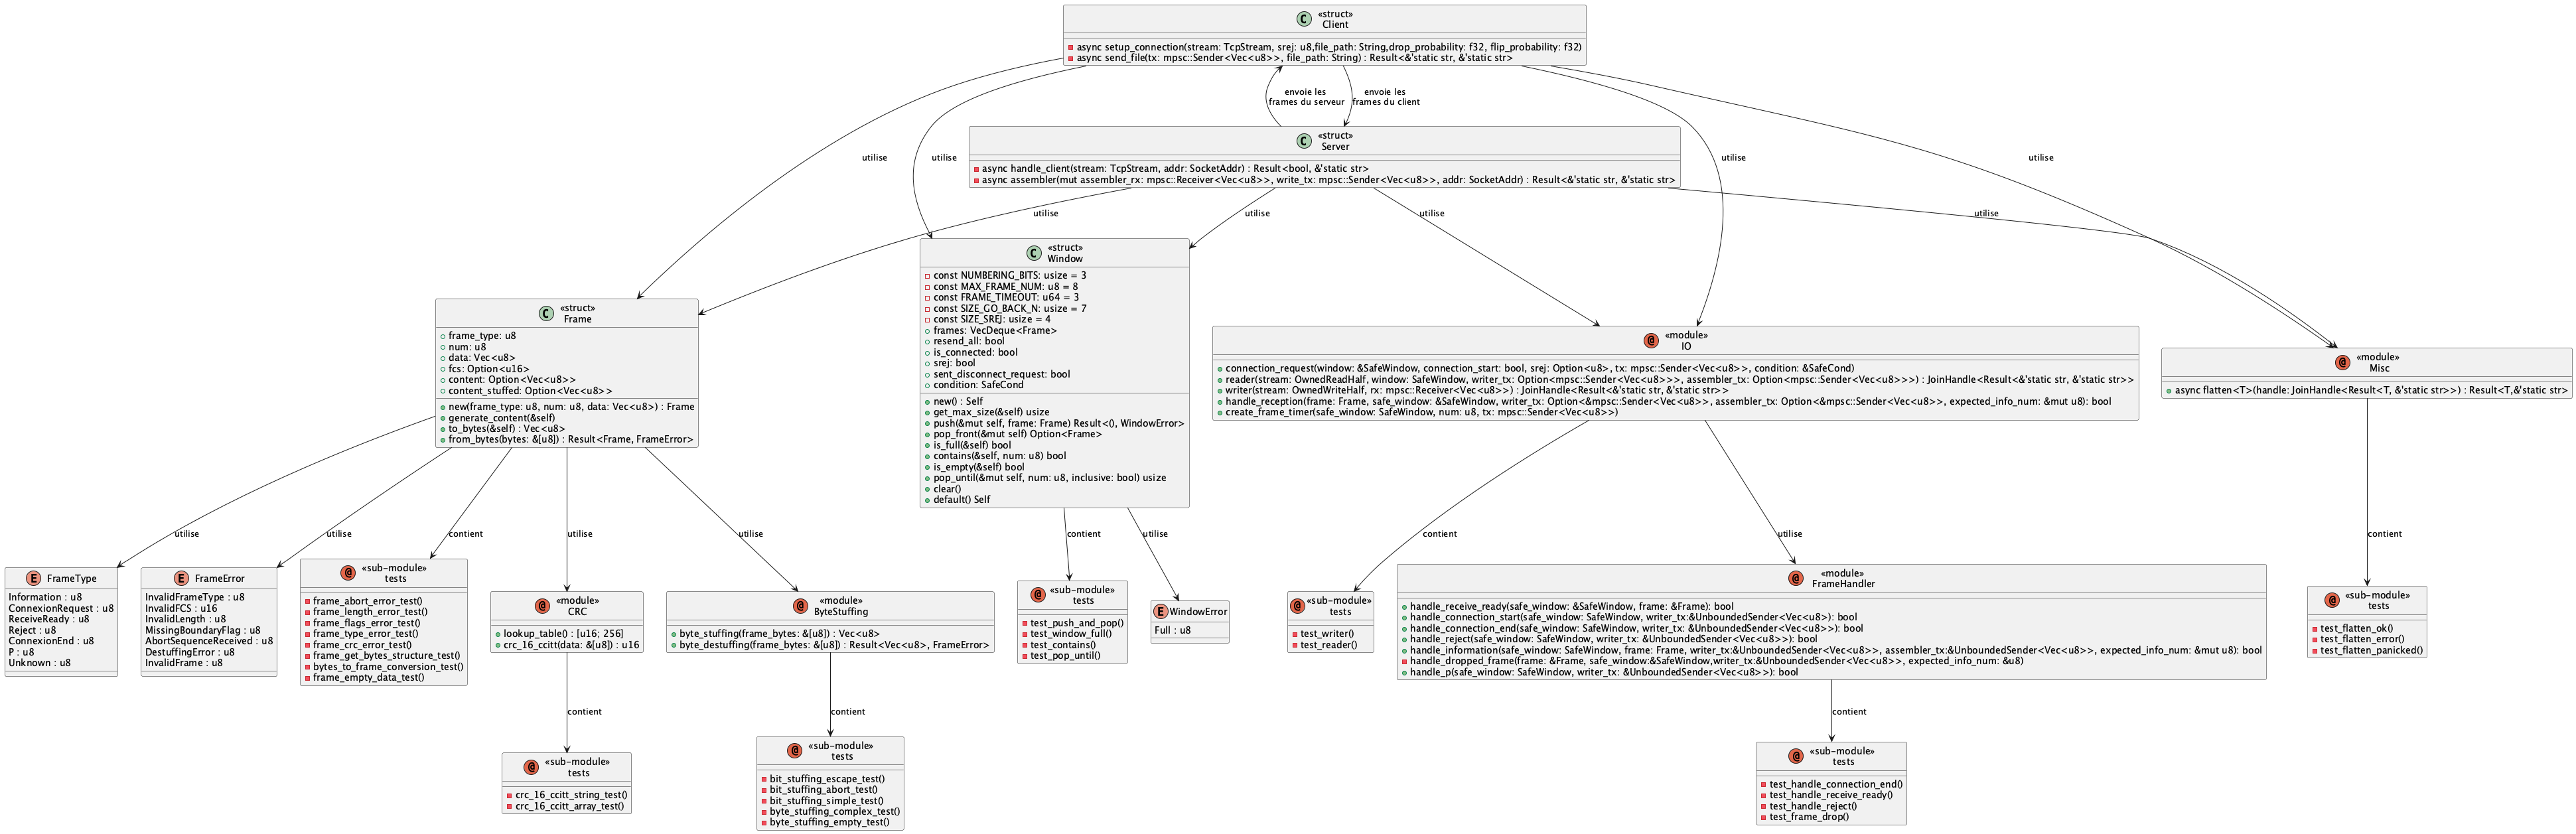
\includegraphics[width=1\textwidth]{../class-diagram/class-diagram.png}
  \caption{Diagramme de classes} 
\end{figure}

Veuillez consulter le fichier \texttt{class-diagram.svg} pour une version plus
lisible du diagramme de classes.

\textbf{Note}: La documentation est présente à l'URL: \href{https://ift3325.etiennecollin.com}{https://ift3325.etiennecollin.com/}

Notre projet se compose de deux modules principaux : le client et le serveur. Commençons par le module client. Ce dernier établit une connexion avec le serveur et initialise deux tâches asynchrones parallèles : le "reader" et le "writer". Chacune de ces tâches prend en charge une "moitié" de la connexion au serveur : le "reader" gère la partie lecture du socket, tandis que le "writer" s'occupe de l'écriture.

Le client envoie une demande de connexion au serveur et attend une réponse. Dès que la réponse est reçue, une troisième tâche asynchrone est lancée. Cette tâche lit le fichier demandé, le divise en morceaux, puis génère des trames à partir de ces morceaux. Les trames sont envoyées dans une fenêtre, tout en veillant à ne pas dépasser sa taille, et sont également transmises au "writer" qui les fait passer par le socket.

Étant donné que plusieurs tâches fonctionnent de manière asynchrone, des mécanismes de synchronisation et de communication sont mis en place pour garantir une bonne interaction entre les différentes parties du système. Pour plus de détails sur le fonctionnement du client, veuillez consulter \href{https://ift3325.etiennecollin.com/client/index.html}{ce lien}.

Le serveur, quant à lui, attend une connexion sur le socket TCP. Une fois la connexion établie, il lance une tâche asynchrone dédiée au traitement du client, permettant ainsi la gestion simultanée de plusieurs clients. Pour chaque client, le serveur démarre deux tâches : "reader" et "writer", comme c’est le cas du côté client.

Cependant, le serveur active également une tâche supplémentaire, appelée "assembler", qui reçoit les trames lues et les réassemble. Ces trames sont lues par le "reader", qui s'assure de vérifier leur intégrité en détectant les trames corrompues ou perdues. Une fois la validité des trames confirmée, celles-ci sont envoyées au "frame handler". Ce dernier prend en charge les opérations spécifiques liées au type de trame reçue.

Lorsqu'une demande de déconnexion du client est reçue, le serveur sait que toutes les données ont été correctement transmises. Il assemble alors le fichier et le sauvegarde avant de fermer le socket. Le serveur est ensuite prêt à accepter de nouvelles connexions. Pour plus de détails sur le fonctionnement du serveur, veuillez consulter \href{https://ift3325.etiennecollin.com/server/index.html}{ce lien}.

Lors de l’utilisation du client et du serveur, une probabilité de perte de trame et de “bit flip” peuvent être spécifiées. Ces opérations servent à simuler une connexion imparfaite et sont appliquées au niveau de la tâche “writer”.

Le module \texttt{Utils} regroupe plusieurs fonctions partagées entre le client et le serveur. Il comprend sept sous-modules, chacun dédié à des fonctions spécifiques. Pour des informations plus détaillées sur les membres du module \texttt{Utils}, consultez \href{https://ift3325.etiennecollin.com/utils/index.html}{ce lien}.

\begin{itemize}
    \item \textbf{Byte Stuffing}: Ce sous-module fournit des fonctions pour le byte stuffing et le byte destuffing. Ces fonctions sont utilisées lors de l'envoi et de la réception de trames par les deux services pour garantir l'intégrité des données transmises.
    \item \textbf{CRC}: Implémentation de l'algorithme CRC-16 CCITT, utilisé pour calculer le CRC d'une trame avant son envoi. Le CRC calculé est ensuite ajouté à la fin de la trame afin de vérifier l'intégrité des données.
    \item \textbf{Frame}: Ce sous-module définit la structure des trames ainsi que des types associés, tels que l'énumération \texttt{FrameType} et \texttt{FrameError}. Il permet de gérer et de manipuler les trames de manière cohérente et typée.
    \item \textbf{FrameHandlers}: Ce sous-module est responsable du traitement des différents types de trames du côté du récepteur. Chaque type de trame (par exemple, RR, Reject, Connexion, Déconnexion, etc.) est géré par une fonction dédiée, assurant une gestion adéquate de tous les scénarios possibles.
    \item \textbf{IO}: Ce sous-module regroupe les fonctions relatives aux opérations d'entrée-sortie (IO), incluant la demande de connexion, la création de temporisations, la gestion de la réception des trames, ainsi que les fonctions reader et writer utilisées pour communiquer via le socket.
    \item \textbf{Misc}: Ce sous-module contient diverses fonctions utilitaires, dont la fonction \texttt{flatten} qui facilite la manipulation des objets \texttt{JoinHandle} asynchrones, permettant ainsi une gestion plus fluide des tâches parallèles.
    \item \textbf{Window}: Ce sous-module est entièrement dédié à la gestion des fenêtres d’envoi et de réception. Il contient tout le code nécessaire pour implémenter la logique des fenêtres, assurant le contrôle de flux et la gestion de la transmission des trames dans un ordre correct.
\end{itemize}

\end{document}
